\section{Auswertung}
\label{sec:Auswertung}
  \subsection{Berechnung der Winkelrichtgröße $D$}
  Um die Winkelrichtgröße $D$ zu bestimmen, wird die Kraft $F$ in Abhängigkeit des Auslenkungswinkels $\varphi$ bei festem Abstand von 
  $0,19975 \,\unit{\meter}$, vermerkt in Tabelle (\ref{tab:F_von_phi}), verwendet. Die Winkelrichtgröße $D$ wird durch Gleichung 
  (\ref{eqn:Winkelrichtgröße}) bestimmt und ist ebenfalls in Tabelle (\ref{tab:F_von_phi}) eingetragen.
  Im Folgenden werden Mittelwerte aus einer Messwerttabelle gebildet. Diese Mittelwerte werden durch 
  $$\bar{x} = \frac{1}{n} \cdot \sum_{i = 1}^{n}x_i$$ berechnet. $n$ ist dabei die Anzahl der Messungen aus welcher der Mittelwert bestimmt wird und
  $x_{i}$ beschreibt die einzelnen Messdaten.
  Der Mittelwertsfehler wird durch 
  $$\Delta \bar{x} = \sqrt{\frac{1}{n \cdot (n - 1)} \cdot \sum_{i = 1}^{n}(x_i - \bar{x})} $$
  berechnet. Bei Größen, die von mehreren fehlerbehafteten Größen abhängig sind, wird die Gaußsche Fehlerfortpflanzung 
  $$\Delta f = \sqrt{\sum_{i = 1}^{n} \left( \frac{\partial f}{\partial x_i} \right)^2 \cdot \left(\Delta x_i \right)^2}$$
  zur Berechnung des Fehlers verwendet. 
  Das mithilfe dieser Formeln gemittelte Ergebnis von $D$ ist 
  $D = (21,0 \pm 0,8) \cdot 10^{-3} \,\,\unit{\newton\meter}$.
  
  \begin{table}[H]
    \centering 
    \caption{Kraft in Abhängigkeit vom Auslenkungswinkel}
    \label{tab:F_von_phi}
    \begin{tblr}{colspec={c c c}}
        \toprule
        $\varphi \,\, [^{\circ}]$ & F [\unit{\newton}] & D [\unit{\newton\meter}]\\
        \midrule
        20 & 0,026 & 0,0149\\
        30 & 0,050 & 0,0191\\
        40 & 0,068 & 0,0195\\  
        50 & 0,090 & 0,0206\\
        60 & 0,120 & 0,0229\\
        70 & 0,136 & 0,0222\\
        80 & 0,156 & 0,0223\\
        90 & 0,184 & 0,0234\\
        100 & 0,200 & 0,0229\\
        110 & 0,210 & 0,0218\\
        \bottomrule
    \end{tblr}
  \end{table}
  

  \subsection{Berechnung des Eigenträgheitmoments}
  Um das Eigenträgheitsmoment der Drillachse $I_{\text{Drill}}$ zu bestimmen, wurde die fünffache Periodendauer $T$ in Abhängigkeit vom Abstand $a$
  bei einer Auslenkung von $90 ^{\circ}$ gemessen. Diese Messwerte sind in Tabelle (\ref{tab:Bestimmung_I_D}) vermerkt. 
  \begin{table}[H]
    \centering 
    \caption{Fünffache Periodendauer $T$ in Abhängigkeit vom Abstand $a$}
    \label{tab:Bestimmung_I_D}
    \begin{tblr}{colspec={c c}}
        \toprule
        $a \,\,[\unit{\meter}]$ & $5 \cdot T \,\,[\unit{\second}]$ \\
        \midrule
        0,050 & 14,40 \\
        0,075 & 16,57 \\
        0,100 & 18,60 \\
        0,125 & 21,41 \\
        0,150 & 30,10 \\
        0,175 & 26,78 \\
        0,200 & 29,94 \\
        0,225 & 32,75 \\
        0,250 & 36,60 \\
        0,300 & 42,50 \\
        \bottomrule
    \end{tblr}
  \end{table}
  $I_{\text{Drill}}$ wird durch die Verbindung $$I_{\text{gemessen}} = I_{\text{Drill}} + 2 \cdot I_{\text{Zh, verschoben}}$$ berechnet. 
  Dabei ist $$I_{\text{Zh, verschoben}} = I_{\text{Zh}} + m \cdot a^2\, ,$$ nach Satz von Steiner (\ref{eqn:SatzVonSteiner}). 
   
  Mithilfe der Gleichung (\ref{eqn:TragheitmomentAusSchwingungsdauer})
  werden $I_{\text{Drill}}$ und $T^2$ durch
  \begin{align}
    I_{\text{Drill}} &= \frac{T^{2} \cdot D}{\left(2 \pi\right)^{2}} - 2 \cdot \left(m \left(\frac{r^{2}}{4} + \frac{h^{2}}{12} \right) + m \cdot a^2 \right) \\
    \Leftrightarrow T^2 &= \frac{8 \pi^2 \cdot m}{D} \cdot a^2 + \frac{4 \pi^2 \cdot I_{\text{Drill}}}{D} + \frac{8\pi^2 \cdot m}{D} \cdot \left( \frac{r^2}{4} + \frac{h^2}{12} \right)
  \end{align}
  ausgedrückt.
  In Abbildung (\ref{fig:plot}) wird $T^2$ gegen $a^2$ aufgetragen und durch lineare Regression der Form $y = m_{\text{St}} \cdot x + n$ werden $m_{\text{St}}$ und $n$ bestimmt.
  $m_{\text{St}}$ beträgt $713,1192 \,\, \unit{\second\squared\per\meter\squared}$ und $n$ beträgt $8,564\,\, \unit{\second\squared}$. 
  \begin{figure}[H]
    \centering
    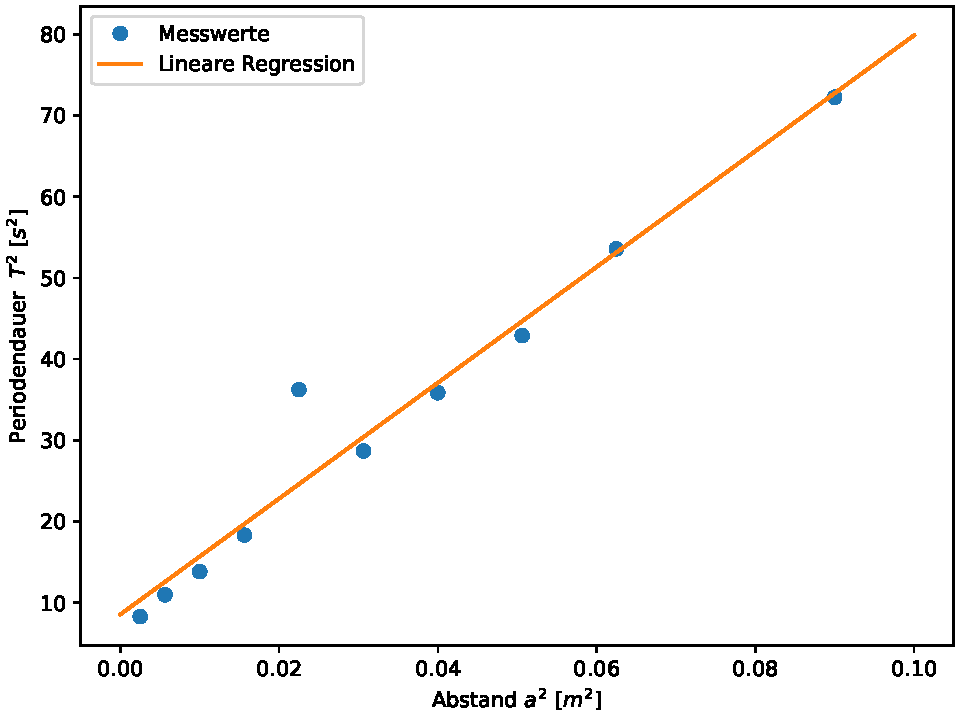
\includegraphics[width=0.95\textwidth]{plot.pdf}
    \caption{Auftragung von Periodenzeit $T^2$ gegen Abstand $a^2$ mit linearer Regression.}
    \label{fig:plot}
  \end{figure}
  Mithilfe dieser Regression und der obigen Gleichung lässt sich das Eigenträgheitsmoment $I_{\text{Drill}}$ mit
  \begin{equation}
    I_{\text{Drill}} = \frac{D \cdot n}{4 \pi^2} - \frac{1}{2} \cdot m \cdot r^2 - \frac{1}{6} \cdot m \cdot h^2
  \end{equation}
  bestimmen. $r$ bezeichnet dabei den Radius und $h$ die Höhe der zylindischen Gewichte, die für die Messung verwendet wurden. Die Messungen dieser beiden
  Größen werden in Tabelle (\ref{tab:Durchmesser_Höhe_Blaues}) und (\ref{tab:Durchmesser_Höhe_Rotes}) aufgeführt. Für die Rechnung wird der Mittelwert beider Gewichte 
   $r = (22,550 \pm 0,010) \cdot 10^{-3}\,\,\unit{\meter}$ und $h = (20,334 \pm 0,008) \cdot 10^{-3} \,\,\unit{\meter}$ verwendet.
  \begin{table}[H]
    \centering 
    \caption{Messungen der Höhe und des Durchmessers des blauen Gewichts}
    \label{tab:Durchmesser_Höhe_Blaues}
    \begin{tblr}{colspec={c c}}
        \toprule
        Höhe $\,[\unit{\meter}]$ & Durchmesser $\,[\unit{\meter}]$ \\
        \midrule
        0,02034 & 0,0450 \\
        0,02030 & 0,0451 \\
        0,02030 & 0,0451 \\
        0,02032 & 0,0451 \\
        0,02030 & 0,0451 \\
        \bottomrule
    \end{tblr}
  \end{table}

  \begin{table}[H]
    \centering 
    \caption{Messungen der Höhe und des Durchmessers des roten Gewichts}
    \label{tab:Durchmesser_Höhe_Rotes}
    \begin{tblr}{colspec={c c}}
        \toprule
        Höhe $\,[\unit{\meter}]$ & Durchmesser $\,[\unit{\meter}]$ \\
        \midrule
        0,02038 & 0,04506 \\
        0,02036 & 0,04510 \\
        0,02032 & 0,04510 \\
        0,02036 & 0,04518 \\
        0,02036 & 0,04516 \\
        \bottomrule
    \end{tblr}
  \end{table}
  Dies ergibt ein Eigenträgheitmoment $I_{\text{Drill}}$ von $(4,46 \pm 0,18) \cdot 10^{-3} \,\,\unit{\kilo\gram\meter\squared}$.

  \subsection{Eigenträgheitmoment der Kugel}
    \subsubsection{Theoretischer Wert}
    Das Eigenträgheitmoment der Kugel $I_{\text{K}}$ wird durch Gleichung (\ref{eqn:TragheitKugel}) berechnet. 
    $r = d / 2$ ist dabei der aus dem Mittelwert der gemessenen Durchmesser berechnete Wert $r = (146,61 \pm 0,20) \cdot 10^{-3} \,\,\unit{\meter}$. 
    Die gemessenen Durchmesser sind in Tabelle (\ref{tab:Durchmesser_Kugel}) dargestellt. $m$ ist $1,1742 \,\,\unit{\kilo\gram}$. 
    
    \begin{table}[H]
      \centering 
      \caption{Gemessene Durchmesser der Kugel}
      \label{tab:Durchmesser_Kugel}
      \begin{tblr}{colspec={c}}
          \toprule
          Durchmesser $\,[\unit{\meter}]$ \\
          \midrule
          0,14660 \\
          0,14590 \\
          0,14660 \\
          0,14685 \\
          0,14710 \\
          \bottomrule
      \end{tblr}
    \end{table}
    Damit beträgt der Theoriewert des Trägheitsmoment der Kugel $I_{\text{K,theo}}$ $(2,524 \pm 0,007) \cdot 10^{-3} \,\,\unit{\kilo\gram\meter\squared}$.
%
    \subsubsection{Gemessener Wert}
    Die für die Rechnung benötigte Periodendauer der Kugel ist in Tabelle (\ref{tab:T5_Kugel}) dargestellt. 
    Diese wurde bei fester Auslenkung um 90° gemessen.
    \begin{table}[H]
      \centering 
      \caption{Gemessene fünffache Periodendauer der Kugel}
      \label{tab:T5_Kugel}
      \begin{tblr}{colspec={c}}
          \toprule
          Periodendauer $\,[\unit{\second}]$ \\
          \midrule
          9,53 \\
          9,50 \\
          9,35 \\
          9,72 \\
          9,40 \\
          9,53 \\
          9,38 \\
          9,31 \\
          9,32 \\
          9,44 \\
          \bottomrule
      \end{tblr}
    \end{table}
    Der Mittelwert einer Periodendauer $T_{\text{K}} = (1,890 \pm 0,008) \,\,\unit{\second}$ wurde für die Berechnung des 
    Trägheitsmomentes $I_{\text{K}}$ mithilfe von Gleichung (\ref{eqn:TragheitmomentAusSchwingungsdauer}) verwendet. \\
    $I_{\text{K}}$ ist $(1,90 \pm 0,08) \cdot 10^{-3} \,\,\unit{\kilo\gram\meter\squared}$.

  \subsection{Eigenträgheitmoment der Scheibe}
    \subsubsection{Theoretischer Wert}
    Das Eigenträgheitmoment der Scheibe wird durch Gleichung (\ref{eqn:TragheitZylinder}) berechnet. $m$ beträgt $0,4237 \,\,\unit{\kilo\gram}$.
    Das zur Berechnung verwendete $r$ wurde aus dem Mittelwert der Messungen des Durchmessers berechnet. 
    Die Messungen der Durchmesser sind in Tabelle (\ref{tab:Durchmesser_Scheibe}) vermerkt. Das mithilfe dieser Werte berechnete, theoretische 
    Trägheitsmoment der Scheibe ist $I_{\text{S,theo}} = (2,552 \pm 0,006) \cdot 10^{-3} \,\,\unit{\kilo\gram\meter\squared}$. 
    \begin{table}[H]
      \centering 
      \caption{Gemessene Durchmesser der Scheibe}
      \label{tab:Durchmesser_Scheibe}
      \begin{tblr}{colspec={c}}
          \toprule
          Durchmesser $\,[\unit{\meter}]$ \\
          \midrule
          0,22010 \\
          0,21890 \\
          0,22010 \\
          0,21920 \\
          0,21915 \\
          \bottomrule
      \end{tblr}
    \end{table}
    \subsubsection{Gemessener Wert}
    Der gemessene Wert des Trägheitmoment der Scheibe $I_{\text{S}}$ wird mithilfe der Gleichung (\ref{eqn:TragheitmomentAusSchwingungsdauer}) berechnet.
    $T = (1,869 \pm 0,006)\,\, \unit{\second}$ ist dabei der Mittelwert der einfachen Periodendauer. Die gemessene fünffache Periodendauer ist in Tabelle (\ref{tab:T5_Scheibe}) dargestellt.
    \begin{table}[H]
      \centering 
      \caption{Gemessene fünffache Periodendauer der Scheibe}
      \label{tab:T5_Scheibe}
      \begin{tblr}{colspec={c}}
          \toprule
          Periodendauer $\,[\unit{\second}]$ \\
          \midrule
          9,28 \\
          9,22 \\
          9,31 \\
          9,34 \\
          9,37 \\
          9,31 \\
          9,56 \\
          9,31 \\
          9,44 \\
          9,31 \\
          \bottomrule
      \end{tblr}
    \end{table}
    Für $I_{\text{S}}$ wird der Wert $(1,85 \pm 0,07) \cdot 10^{-3} \,\,\unit{\kilo\gram\meter\squared}$ berechnet. 
     
  
  \subsection{Trägheitsmoment der Puppe}
    \subsubsection{Position 1 der Puppe}
      \textbf{Theoretischer Wert}\\
        Zur Berechnung des Trägheitsmoments der Puppe in Position 1 werden eine Reihe von Vereinfachungen angenommen. Der Kopf wird genauso
        wie die Arme, Beine und der Torso als zylindrisch angenommen und die Dichte als homogen. Der Durchmesser der einzelnen Zylinder wird 
        als Mittelwert der Messungen der Durchmesser angenommen. Diese Messungen sind in Tabelle (\ref{tab:Durchmesser_Puppe}) aufgeführt. 

        \begin{table}[H]
          \centering 
          \caption{Gemessene Durchmesser der einzelnen Puppenteile}
          \label{tab:Durchmesser_Puppe}
          \begin{tblr}{colspec={c c}}
              \toprule
              Kopf $\,\,[\unit{\meter}]$ & Arm $\,\,[\unit{\meter}]$ & Torso $\,\,[\unit{\meter}]$ & Bein $\,\,[\unit{\meter}]$\\
              \midrule 
              0,02726 & 0,00824 & 0,02330 & 0,01900 \\
              0,02786 & 0,01480 & 0,02708 & 0,01734 \\
              0,01510 & 0,01200 & 0,03874 & 0,01178 \\
              0,01650 & 0,01412 & 0,03230 & 0,01514 \\
              0,02300 & 0,01520 & 0,03834 & 0,01694 \\
              & 0,01138 & 0,04230 & 0,01304 \\
              & 0,01270 & 0,04020 & 0,00924 \\
              & 0,01020 & 0,03600 & 0,01708 \\
              & 0,01180 & 0,03472 & 0,01620 \\
              & 0,01384 & 0,03800 & 0,01344 \\
              \bottomrule
          \end{tblr}
        \end{table}
        Mithilfe der gemittelten Durchmesser $d_{\text{Kopf}} = (21,9 \pm 2,7) \cdot 10^{-3}\,\,\unit{\meter}$,
         $d_{\text{Arm}} = (12,4 \pm 0,7) \cdot 10^{-3}\,\,\unit{\meter}$,
          $d_{\text{Torso}} =  (35,1 \pm 1,9)\cdot 10^{-3}\,\,\unit{\meter}$ und
          $d_{\text{Bein}} = (14,9 \pm 0,9)\cdot 10^{-3}\,\,\unit{\meter}$ 
          werden die Volumina der einzelnen Körperteile berechnet, um dadurch die Masse der Einzelteile zu bestimmen. 
        Bei dieser Berechnung wird angenommen, dass die Dichte der Puppe homogen ist. Die Volumina der Puppenteile werde durch  
        $$V = \pi \cdot r^2 \cdot h$$
        berechnet. $r$ ist dabei der Radius der Zylinder und $h$ die Höhe. 
        Das berechneten Volumen der Puppenteile, sowie die daraus anteilig am Gesamtgewicht von $0,1696 \,\,\unit{\kilo\gram}$ bestimmte Massen sind in Tabelle (\ref{tab:Volumen_Puppe}) 
        und (\ref{tab:Massen_Puppe}) gelistet. 
        \begin{table}[H]
          \centering 
          \caption{Volumina der Puppenteile}
          \label{tab:Volumen_Puppe}
          \begin{tblr}{colspec={c c c c}}
              \toprule
              Kopf $\,[10^{-5}\,\,\unit{\meter\tothe{3}}]$ & Arm $\,[10^{-5}\,\,\unit{\meter\tothe{3}}]$ & Torso $\,[10^{-5}\,\,\unit{\meter\tothe{3}}]$ & Bein $\,[10^{-5}\,\,\unit{\meter\tothe{3}}]$\\
              \midrule 
              2,0 \pm \,\, 0,5 & 1,66 \pm \,\,0,18 & 10,0 \pm \,\,1,0 & 3,0 \pm \,\,0,4 \\
              \bottomrule
          \end{tblr}
        \end{table}

        \begin{table}[H]
          \centering 
          \caption{Massen der Puppenteile}
          \label{tab:Massen_Puppe}
          \begin{tblr}{colspec={c c c c}}
              \toprule
              Kopf $\,[\unit{\kilo\gram}]$ & Arm $\,[\unit{\kilo\gram}]$ & Torso $\,[\unit{\kilo\gram}]$ & Bein $\,[\unit{\kilo\gram}]$\\
              \midrule 
              0,017 \pm\, 0,004 & 0,0136 \pm\, 0,0015 & 0,078 \pm\, 0,006 & 0,0242 \pm\, 0,0026 \\
              \bottomrule
          \end{tblr}
        \end{table}
        Mithilfe dieser Massen wird das Trägheitsmoment der einzelnen Puppenteile bestimmt, woraus sich das Gesamtträgheitsmoment der Puppe in 
        Position 1 zusammensetzt. Da alle Gliedmaße als Zylinder genähert wurden, werden die Trägheitsmoment durch Formel (\ref{eqn:TragheitZylinder})
        für den Kopf, den Torso und die Beine und Formel (\ref{eqn:TrägheitZylinderQuer}) für die vom Torso ausgestrecken Arme berechnet. 
        Für die Berechnung des Trägheitsmomentes der Beine und Arme wird der Satz von Steiner angewandt. Der dabei verwendete Abstand beträgt bei den 
        Beinen näherungsweise den Radius der Beine und bei den Armen die Summe aus dem Radius des Torsos und der Hälfte der Höhe der Arme. 
        Diese Werte führen zu einem theoretischen Trägheitsmoment der Puppe in Position 1 $I_{\text{Pos1,theo}}$ von $(0,262 \pm 0,025) \cdot 10^{-3}\,\, \unit{\kilo\gram\meter\squared}$.
        \\
        \\
      \textbf{Gemessener Wert} \\
      Die gemessenen, fünffachen Periodendauern der Puppe in Position 1 sind in Tabelle (\ref{tab:T5_Positon_1}) vermerkt, unterschieden 
      nach Auslenkung um $90$° und $120$°. 
      \begin{table}[H]
        \centering 
        \caption{Fünffache Periodendauer der Puppe in Position 1}
        \label{tab:T5_Positon_1}
        \begin{tblr}{colspec={c c}}
            \toprule
            T bei Auslenkung um 90° $\,\,[\unit{\second}]$ & T bei Auslenkung um 120° $\,\,[\unit{\second}]$ \\
            \midrule
            3,10 & 3,15 \\
            3,06 & 3,06 \\
            3,06 & 3,19 \\
            3,03 & 3,00 \\
            3,03 & 3,03 \\
            \bottomrule
        \end{tblr}
      \end{table}
      Da der Mittelwert der Periodendauer bei Auslenkung um $90$° und $120$° annähernd gleich sind, wird davon ausgegangen, dass keine Abhängigkeit der 
      Periodendauer von der Auslenkung besteht und beide Messungen zusammengefasst betrachtet werden können. 
      Der allgemeine Mittelwert der Periodenauer $T$ ist daher $T = 0,614 \pm 0,004\,\, \unit{\second}$. 
      Mithilfe dieses Mittelwertes und Formel (\ref{eqn:TragheitmomentAusSchwingungsdauer}) wird das 
      Trägheitsmoment der Puppe in Position 1 $I_{\text{Pos1}}$ berechnet. 
      $I_{\text{Pos1}}$ ist $(0,2 \pm 0,008) \cdot 10^{-3}\,\, \unit{\kilo\gram\meter\squared}$.
            
    \subsubsection{Position 2 der Puppe}
    Bei Position 2 der Puppe wurde vereinfachend angenommen, dass beide Beine im Winkel von $90$° vom Torso wegzeigen. 
    Die Armposition ist dieselbe wie bei Position 1 der Puppe.\\
    \\
      \textbf{Theoretischer Wert} \\
      Für die Berechnung des theoretischen Wertes des Trägheitsmoments der Puppe in Position 2 werden die bereits berechneten Trägheitsmomente der
      Arme, des Kopfes und des Torsos übernommen, da deren Positionen keine Veränderung aufweist. 
      Neu berechnet werden hingegen die Trägheitsmomente der Beine. Für die Berechnung dieser wird Formel (\ref{eqn:TrägheitZylinderQuer}) und
      der Satz von Steiner verwendet. 
      Das theoretisch berechnete Trägheitsmoment der Puppe in Position 2 $I_{\text{Pos2,theo}}$ beträgt demnach $(0,72 \pm 0,05) \cdot 10^{-3}\,\, \unit{\kilo\gram\meter\squared}$. \\
      \\
      \textbf{Gemessener Wert} \\
      Wie bereits bei Position 1 festgestellt, hängt die Periodendauer nicht von der Auslenkung ab. Daher werden auch bei Position 2 beide Messwertreihen
      zusammen betrachtet. Die gemessene fünffache Periodendauer ist trotzdessen in Tabelle (\ref{tab:T5_Positon_2}) nach Auslenkungswinkel 
      getrennt aufgeführt.
      \begin{table}[H]
        \centering 
        \caption{Fünffache Periodendauer der Puppe in Position 2}
        \label{tab:T5_Positon_2}
        \begin{tblr}{colspec={c c}}
            \toprule
            T bei Auslenkung um 90° $\,[\unit{\second}]$ & T bei Auslenkung um 120° $\,[\unit{\second}]$ \\
            \midrule
            4,72 & 4,85 \\
            4,87 & 4,90 \\
            4,84 & 4,81 \\
            4,69 & 4,87 \\
            4,69 & 4,85 \\
            \bottomrule
        \end{tblr}
      \end{table}
      Der Mittelwert der Periodenauer $T$ ist $T = (0,962 \pm 0,004)\,\, \unit{\second}$. 
      Mithilfe dieses Mittelwertes und Formel (\ref{eqn:TragheitmomentAusSchwingungsdauer}) wird das 
      Trägheitsmoment der Puppe in Position 2 $I_{\text{Pos2}}$ berechnet. 
      $I_{\text{Pos2}}$ ist $ (0,491 \pm 0,020) \cdot 10^{-3}\,\, \unit{\kilo\gram\meter\squared}$.
        

  
%Siehe \autoref{fig:plot}!